% LREC-COLING 2024 Example; 
% LREC Is now using templates similar to the ACL ones. 
\documentclass[10pt, a4paper]{article}

\usepackage{lrec-coling2024} % this is the new style

\usepackage{fontspec}
\setmainfont{Arial}
\usepackage{listings}

\usepackage{natbib}
\usepackage{multibib}
\makeatletter
%\def\@mb@citenamelist{cite,citep,citet,citealp,citealt,citepalias,citetalias}
\makeatother
\newcites{languageresource}{~}
\renewcommand{\refname}{{}}
\usepackage{graphicx}
\usepackage{tabularx}
\usepackage{soul}
% for eps graphics
%%% References and Labels
%%% Reference labels without a punctuation 
% courtesy of Marc Schulder , uni Hamburg ****************
\usepackage{titlesec}
%\titleformat{\section}{\normalfont\large\bf\center}{\thesection.}{1em}{}
\titleformat{\section}{\normalfont\large\bfseries\center}{\thesection.}{1em}{}
\titleformat{\subsection}{\normalfont\SmallTitleFont\bfseries\raggedright}{\thesubsection.}{1em}{}
\titleformat{\subsubsection}{\normalfont\normalsize\bfseries\raggedright}{\thesubsubsection.}{1em}{}
\renewcommand\thesection{\arabic{section}}
\renewcommand\thesubsection{\thesection.\arabic{subsection}}
\renewcommand\thesubsubsection{\thesubsection.\arabic{subsubsection}}
%  ed 

\usepackage{microtype}
\usepackage{todonotes}
\usepackage{booktabs}
\usepackage{paralist}
\usepackage{colortbl}

\usepackage{xcolor}
\usepackage{hyperref}
 \definecolor{darkblue}{rgb}{0, 0, 0.5}
  \hypersetup{colorlinks=true, citecolor=darkblue, linkcolor=darkblue, urlcolor=darkblue}

\usepackage{xstring}

\usepackage{color}

\newcommand{\secref}[1]{\StrSubstitute{\getrefnumber{#1}}{.}{ }}

\title{Are Sounds Sound for the Reconstruction of Language Trees? Comparing Lexical Cognates and Sound Correspondences in Bayesian Phylogenetic Inference}

\name{} 

\address{ \\ \\ \\}% Affiliation1, Affiliation2, Affiliation3 \\
%         Address1, Address2, Address3 \\
%         author1@xxx.yy, author2@zzz.edu, author3@hhh.com\\
%         \{author1, author5, author9\}@abc.org\\}


\abstract{ In traditional studies on language evolution, scholars often emphasize the important role which sound laws and sound correspondences play in the task of reconstructing the phylogeny of a language family. However computational approaches have largely ignored the potential importance of sound laws and sound correspondences.  Most computational studies still employ lexical cognates as the major data when it comes to phylogenetic reconstruction in linguistics, although there are a few studies in which authors praise the benefits of comparing words at the level of sound sequences. Building on (a)~ten diverse datasets from different language families, and (b)~state-of-the-art methods for automated cognate and sound correspondence detection, we test, for the first time, the performance of sound-based versus cognate-based approaches to phylogenetic reconstruction.  Our results show that phylogenies reconstructed from lexical cognates tend to come closer to gold standard phylogenies than phylogenies reconstructed from sound correspondences.  \\ \newline \Keywords{sound correspondences, phylogenetic reconstruction lexical cognates}%
}

\begin{document}

\maketitleabstract%
%
\section{Introduction}

Although controversially discussed in the beginning \citep{Holm2007}, quantitative approaches to phylogenetic reconstruction based on Bayesian phylogenetic inference frameworks have now become broadly accepted in the field of comparative linguistics. This is reflected in more and more computer-based phylogenies that have been proposed for the world's largest language families---Dravidian \citep{Kolipakam2018}, Sino-Tibetan \citep{Sagart2019} and Indo-European \citep{bouckaert2012mapping}---and even fully automated workflows have shown to be quite robust \citep{rama2018automatic}.  While rarely practiced in the pre-computational past of historical linguistics, computing detailed phylogenies has now become one of the key tasks of studies on language evolution.


Although traditional scholars have started to accept computational language phylogenies as a new tool deserving its place in the large tool chain of comparative linguistics, scholars still express a lot of skepticism against the idea of most of the language phylogenies that have been proposed so far. One of the major reasons usually mentioned in this context is that phylogenetic approaches are usually based on cognate sets (sets of historically related words) identified in semantically aligned word lists. Since these \emph{cognate sets} reflect \emph{lexical data} only, many scholars mistrust them, given that lexical data are assumed to be much less stable than other aspects of languages~\cite{CampbellPoser2008}.
 
In classical historical linguistics, the data used for subgrouping are traditionally composed of small collections of so-called \emph{shared innovations} \citep{Dyen1953}. What counts as a shared innovation has itself never been well-defined in the literature, but the largest amount of data used by scholars is traditionally taken from sound correspondences or supposed sound change processes (compare, for example the data in \citealt[305]{Anttila1972}). Although it is controversially debated in the field \citep{Ringe2002,Dybo2008}, many classical linguists still emphasize that sound correspondences are largely superior to lexical data when it comes to subgrouping.

There have only been a few attempts to test how well quantitative approaches to phylogenetic reconstruction perform when using sound correspondences instead of lexical cognates \citep{Chacon2015a}. The main reason is that coding data to compute phylogenies from sound change data is very tedious even for a dataset with 20 languages.  For this reason, there have only been a few attempts to test how well quantitative approaches to phylogenetic reconstruction perform when using sound correspondences instead of lexical cognates.
% \citep{Chacon2015a}. 

Building on the state-of-the-art methods for automatic cognate detection and phonetic alignment in historical linguistics \citep{List2016g}, combined with novel approaches for the inference of sound correspondence patterns in multilingual datasets \citep{List2019a} and customized solutions for phylogenetic reconstruction \citep{Rama2019} that have evolved into a new Python library for phylogenetic inference, we have been able to create a new workflow for phylogenetic reconstruction based on sound correspondence patterns.  With a new collection of ten gold standard datasets, we test the workflow and compare it with alternative workflows based on lexical data alone. Our results indicate that sound correspondence patterns are far less suitable for the purpose of computer-based phylogenetic reconstruction than expected.

% The contributions\todo{The contributions as pointed by the reviewer.} of the paper are as followed:

% \begin{itemize}
%     \item A new implementation of phylogenetic inference software
%     \item automating sound-based representations and alignment
%     \item evaluating sound vs. lexical information
% \end{itemize}



%In this paper, we test if word aligned data be useful for phylogenetic inference for datasets ranging from dialects to languages. Do correspondence set algorithms reduce the ambiguity in the data which in turn can be used for inferring trees? Do multi-state characters perform better than binarized aligned data? In the face of uncertainty regarding the type of data, which level of data should be employed for phylogenetic inference? In the process of answering these questions, we developed and tested new phylogenetic inference software that uses a new algorithm known as serial tempering for navigating the tree space. We make all our data and code available with the paper.

\section{Background}\label{sec:motiv}

Much of the previous work on phylogenetic reconstruction using Bayesian phylogenetic inference~\cite{Kolipakam2018,Sagart2019,rama2018automatic} is based on cognate sets encoded as binary vectors, where the presence or absence of a language in a cognate set is coded as \textbf{0} or \textbf{1}, and phylogenetic trees are inferred by assuming that cognate sets evolve along a phylogenetic tree in the form of gain and loss processes (see Figure~\ref{fig:1}).

\begin{figure}[tb!]
    \centering
    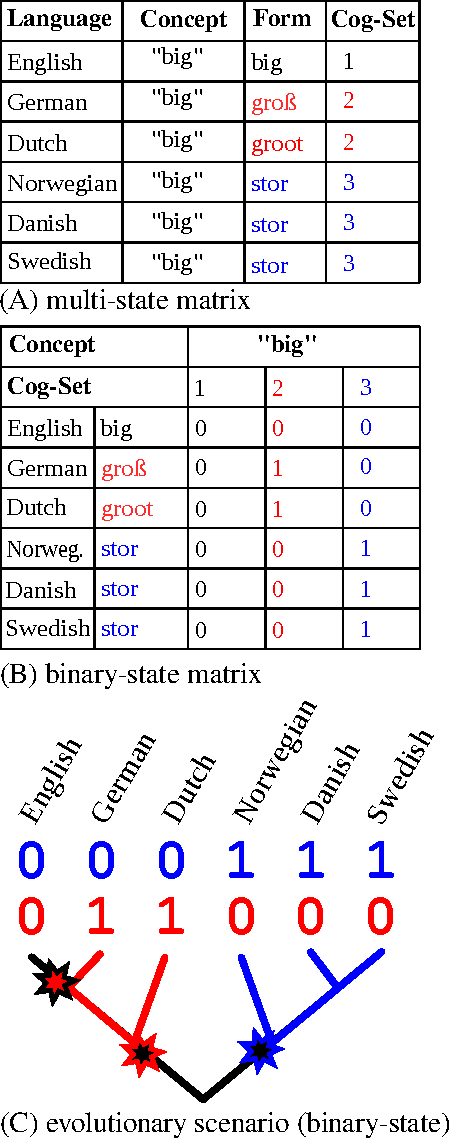
\includegraphics[width=0.4\textwidth]{figures/figure-1.pdf}
    \caption{Gain-loss processes derived from binary cognate vectors. A shows a wordlist in which
    cognate words are coded in multi-state fashion. B shows the corresponding binary coding. C shows
    how gain and loss processes are modeled on a phylogenetic tree.}\label{fig:1}
\end{figure}


The binary-state coding is the most frequently applied coding technique, and it is being used in this study as well. Once assembled, binary state data can be modeled with binary state Continuous Time Markov Chain model (\emph{binary-CTMC}, \citealt{bouckaert2012mapping}), which allow gain and loss processes to occur an arbitrary number of times. 

The \textit{major contributions} of this study are:
\begin{inparaenum}[(1)]
\item we 
provide an automated workflow that 
allows
to infer cognates and correspondence patterns and analyze them with
the help of Bayesian phylogenetic inference methods, implemented in a new software package,

\item we show how the quality of phylogenetic reconstruction approaches based on sound correspondences can be compared to phylogenetic reconstruction based on lexical data, and in this way
\item we put the debate about the usefulness of sound-based as opposed to cognate-based phylogenies to the test.
\end{inparaenum}


As an early example for sound-based approaches to phylogenetic reconstruction, \citet{hruschka2015detecting} apply a CTMC model that allows transitions between a fixed number of sounds for detecting the important sound changes in a dataset consisting of etymologies across Turkic languages. The authors do not infer phylogenies from their data but rather use an established phylogeny (which are not readily available for many language families of the world) to infer branch lengths and transition probabilities between sounds in their data in order to detect sound changes at different time points in a time-calibrated family tree of Turkic. 

\citet{Wheeler2015b} start from typical word lists (that would otherwise be used in phylogenetic reconstruction based on lexical data) and apply a parsimony-based algorithm that aligns words regardless if they are cognate or not, reconstructs a hypothetical ancestral word from the alignment, and seeks to infer the phylogeny that allows to explain the sequences by a minimal amount of assumed transitions \citep{Sankoff1975}. In a later study, \citet{Whiteley2019} apply the same approach to a dataset of Bantu languages. The method by \citet{Wheeler2015b} is linguistically flawed, since words are not assigned to cognate sets before aligning them. It is well known that there is a strict difference between regular sound change processes and processes resulting from lexical replacement \citep{Hall2010} and that even words that are cognate are not necessarily fully \emph{alignable}
\citep[10]{Schweikhard2020}.


\citet{Chacon2015a} start from manually extracted sound correspondence patterns for consonants in a dataset of 21 Tukanoan languages, to which proto-forms had also been added manually. Based on the sound correspondence patterns, they apply---similar to \citet{Wheeler2015b}---an algorithm that searches for the tree that provides the most parsimonious scenario for the evolution of the sounds. In contrast to \citet{Wheeler2015b}, however, they added specific constraints for the transitions from one sound to another sound, which were based on expert judgments for the Tukanoan language family. The approach by \citet{Chacon2015a}, finally, requires an enormous amount of preprocessing that runs the risk of leading to circular results, since proto-forms and major directions of sound change processes are required to be known in advance. While all approaches have their individual shortcomings, one of the largest shortcomings lies in the fact that it is very difficult to apply them. This is also witnessed by the fact that no additional studies have been carried out by other teams, although all the methods have been proposed years ago.


\section{Materials and Methods}

\subsection{Materials}

\begin{itemize}
\item describe datasets (table)
\item describe preprocessing 
\item describe binarization 
\end{itemize}


\subsection{Methods}

mostly gerhard on trees, etc.

\subsection{Evaluation}

mostly gerhard on trees

\subsection{Implementation}

Mattis + Gerhard

\section{Results}

Gerhard + mattis comments

\section{Discussion and Conclusion}

\section{Supplementary Material}





\bibliographystylelanguageresource{lrec_natbib}
\bibliographylanguageresource{languageresource}

\bibliographystyle{lrec_natbib}
\bibliography{languageresource}

\newpage

\end{document}

%%% Local Variables:
%%% mode: xelatex
%%% TeX-master: t
%%% End:
